\chapter{Designing Privacy Enhancing Tools Comparison Environment}
\label{chapter-4}

As outlined in Chapter~\ref{chapter-2}, multiple methods for user tracking exist. Consequently, privacy-preserving tools that prevent tracking have been developed. However, these tools are mainly independent of each other and thus differ in both the~anti-tracking methods they provide and their effectiveness.

Since not all anti-tracking tools have their source code publicly available, comparing their functionality by studying the~code is impossible.
Consequently, specialized solutions have been developed to compare their effectiveness. Several of these solutions are described in Chapter~\ref{chapter-3}. The~main objective of this thesis is to improve existing comparisons of anti-tracking tools. This chapter presents a~testing environment and the~comparisons that will be performed since they are the~primary focus of this thesis.

\section{Environment and Comparison System Design}

To design an~environment for the~comparisons, it is first necessary to establish the~requirements. The~basic requirements are summarized in the~following list:

\begin{itemize}
    \setlength\itemsep{0em}
    \item The~environment should be documented and easy to replicate.
    \item The~environment should support multiple anti-tracking tools.
    \item The~environment should support the~addition of new tools developed in the~future.
    \item Comparison methods should be clearly defined, accompanied by their respective limitations.
    \item Comparison methods should be deterministic, making the~results replicable.
\end{itemize}

One of the~requirements for the~environment is to ensure its replicability, which can be accomplished by employing the~technologies presented in Section~\ref{EnvironmentSection}. However, the~environment could also be set up manually by following steps that prepare a~system to support the~comparison methods. Furthermore, the~environment should support multiple anti-tracking tools, including existing tools presented in Section~\ref{Section-Anti-tracking}, and additional tools that may emerge. Overall, the~environment only serves as a~container for the~proposed comparison methods.

Selected methods of comparing anti-tracking tools are described in Section~\ref{existing-tools-methods}. \textit{OpenWPM} is a~tool often used in existing anti-tracking research~\cite{petranova-bit, iqbal2020fingerprintingfingerprinterslearningdetect, comparison-mazel}. While OpenWPM is explicitly designed for web privacy research and is still maintained even in 2024, it lacks one crucial feature: the~support of other browsers. OpenWPM can only be used with the~Firefox browser, which is insufficient for this thesis, as it also aims to compare the~anti-tracking performance of different browsers presented in Section~\ref{Section-Anti-tracking}. Alternative comparison tools are usually outdated or incompatible with the~stated requirements. Thus, a~custom system needs to be designed. However, the~system adapts and integrates certain concepts and approaches from existing solutions.

\section{Proposed Evaluation Methods}
\label{comparison-methods-label}

Following a~discussion with the~thesis supervisor, this work focuses only on evaluating content blockers, i.e., privacy-enhancing tools that block network requests for content that may also include trackers. This section describes two proposed evaluation methods. There are many approaches to evaluate the~effectiveness of content blockers. However, no single comparison can definitively determine which tool is the~most effective. While the~methods presented here aim to provide meaningful insights, it is essential to understand the~inherent limitations of each approach.

\subsection{Ensuring Determinism Across Evaluations}
It is necessary to compare the~content blockers on the~same dataset for a~fair and deterministic comparison. Simply visiting a~set of pages multiple times to test different content-blocking tools does not ensure determinism, as the~pages may request different content each time they are visited.

Because of this variability, comparing the~number of blocked requests across multiple page visits can be misleading. One tool might appear more effective simply because it encountered more blockable requests, not because it is inherently better at blocking them. For instance, a~request to a~specific tracker might be present in one test run but not in another, which would unfairly skew the~results.

This issue of non-determinism can be partially mitigated by increasing the~number of page visits. For example, Mazel et al.~\cite{comparison-mazel} visited each page multiple times and averaged the~results to smooth out inconsistencies. However, this still does not guarantee determinism.

A truly deterministic approach involves capturing and saving the~network traffic from each visited page to build a~consistent dataset. Once this dataset is created, it can be replayed with different content-blocking tools under the~same conditions. This allows for a~deterministic comparison, as each tool can block the~same set of requests.

\subsection{Evaluation of Requests Blocked by Content-Blocking Tools}
\label{comparison-3}
The first evaluation method measures how effectively each content blocker prevents outgoing network requests by calculating the~number of blocked requests from a~given dataset. It also considers the~structure of the~requests, accounting for cases where one request depends on another.

\subsubsection{Performance Metrics}
A simple comparison might rely on the~built-in reports from each tool. However, such an~approach is unreliable since the~reports may not be precise, or the~tool might not provide any reports at all. Thus, such a~comparison is not feasible. Instead, a~custom evaluation system is used, applying uniform metrics across all tools. Requests are replayed using the~previously mentioned dataset, and the~number of requests blocked by each tool can be directly compared, as the~blockings occurred on the~same data.

\subsubsection{Tree-like Request Structure}

However, a~simple comparison of the~number of blocked requests still presents a~problem: web requests often have a~tree-like structure. Therefore, some requests act as the~entry point of other requests, meaning that blocking one parent request may prevent many child requests. For example, suppose a~user visits page \emph{A}, which includes a~tracker from page \emph{B}. \emph{B} may then load additional content from \emph{C} and \emph{D}. Consequently, when a~user visits page \emph{A}, pages \emph{B, C} and \emph{D} are also requested.

Two requests are marked as blocked if one content blocker blocks \emph{C} and \emph{D}. Another tool might only block page \emph{B}, thereby also transitively preventing requests for \emph{C} and \emph{D}. However, this second tool only blocked one request, even though its action effectively blocked three requests. A~simplistic count would incorrectly suggest that the~first tool was more effective in such a~scenario.

The evaluation preserves the~directed request tree to address the~abovementioned issue. Figure~\ref{domain-tree} illustrates a~simple request tree. The~tree structure has been used to model request relations before. For example, Sanchez-Rola et al.~\cite{iskander-cookies} used a~tree-like structure to model how requests create cookies. The~parent-child relations between requests are obtained from the~network logs. If a~parent request is blocked, all its children are also considered blocked, which more accurately reflects the~impact of blocking a~request.

\begin{figure}[!ht]
    \centering
    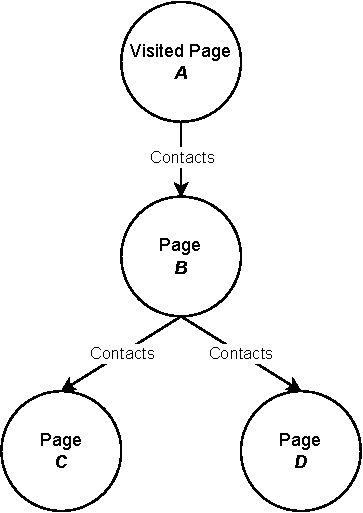
\includegraphics[scale=1]{obrazky-figures/domain_tree.pdf}
    \caption[Illustration of a~tree-like request chain]{Illustration of a~tree-like request chain which allows for accurate measurement of number of requests blocked.}
    \label{domain-tree}
\end{figure}

\subsubsection{Limitations}
Despite its advantages, this evaluation has limitations. It only reflects behavior based on the~pages and resources that were observed.
Consequently, it is impossible to determine how the~extension would behave on unvisited pages, which may contain different requests. 

Another limitation lies in the~subjectivity of filter lists, as discussed in Section~\ref{existing-blacklists}. These lists are created by people, often with different priorities. For example, a~tool might block more requests simply because its filter lists include more pages, even though other people would not block these requests. Therefore, a~higher number of blocked requests does not necessarily imply one tool is better than another. A~deeper analysis would require manual inspection of blocked requests to ascertain the~validity of the~blocking action. Even so, this evaluation method still offers insight into the~general behavior of different content-blocking tools.


\subsection{Evaluation of Anti-Tracking Capabilities of Content-Blocking Tools}
\label{content-blocking-design}
The second method builds on the~previous one by focusing on the~anti-tracking capabilities of the~content blockers. It measures how many JavaScript fingerprinting API calls were blocked due to blocking the~resources that attempted to initiate them. These calls can reveal unique information about the~user’s browser and device, as discussed in Subsection~\ref{browser-fingerprinting}.


\subsubsection{Observing Fingerprinting API Calls}
The JShelter browser extension, presented in Subsection \ref{jshelter-introduction}, can be used to capture the~API calls. JShelter includes a~Fingerprint Detector based on Marek Saloň’s master’s thesis~\cite{salon-mit}, which can detect the~calls of APIs misused for fingerprinting in real-time. These API calls represent potential fingerprinting attempts since they may be used in the~fingerprint calculation process.

No content blockers are active during the~dataset creation, and JShelter’s protections are disabled to avoid interference. The~Fingerprint Detector logs fingerprinting API calls on each visited page, which can be matched with the~associated network traffic logs.


\subsubsection{Performance Metrics}
This evaluation intends to quantify the~anti-tracking capabilities of a~given content-blocking tool. It uses the~same tree-like request structure described in the~previous evaluation in Subsection~\ref{comparison-3}, but with additional information. Each node (i.e., each contacted resource) is assigned the~number of fingerprinting API calls it caused during the~visit. This allows using request trees and their transitive properties to obtain the~number of fingerprinting attempts that could be prevented by blocking a~specific request.

For example, if page \emph{A} loads page \emph{B}, which then loads \emph{C} and \emph{D}, and fingerprinting attempts are observed on all of them, a~content blocker that blocks \emph{B} would also prevent the~subsequent calls from \emph{C} and \emph{D} as they would not be loaded. This would reduce the~total number of fingerprinting API calls by all the~calls caused by pages \emph{B, C} and \emph{D}. Figure~\ref{domain-api} illustrates a~request tree with associated fingerprinting attempts.


\begin{figure}[!ht]
    \centering
    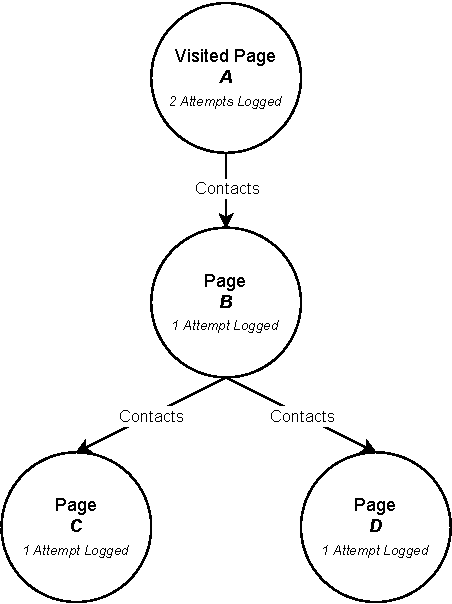
\includegraphics[scale=0.92]{obrazky-figures/domain-api.pdf}
    \caption[Illustration of a~request tree with fingerprinting attempts caused by each node]{Illustration of a~request tree where each node is assigned its API calls that can be misused for fingerprinting.}
    \label{domain-api}
\end{figure}

\subsubsection{Limitations}
This method inherits the~limitations of the~first evaluation. Additionally, it cannot confirm whether observed fingerprinting API calls were used for tracking. These APIs have legitimate uses, so not all calls represent tracking behavior. Consequently, blocking more API calls that are potentially usable for fingerprinting might not be inherently better than blocking less. However, this evaluation still provides a~way to compare how well different tools prevent potential fingerprinting, complementing the~first request-based evaluation with a~more privacy-oriented metric.
